%% Installer les paquets texlive-lang-french et texlive-fonts-recommended pour pouvoir compiler ce document
\documentclass{article}
\usepackage{geometry}
\geometry{
	a4paper,
	left=20mm,
	right=20mm,
	top=30mm,
	bottom=40mm,
}
\usepackage[utf8]{inputenc}
\usepackage[T1]{fontenc}
\usepackage[french]{babel}
\usepackage{graphicx}

\begin{document}

\title {Rapport Projet NachOS \\ M1 Informatique}
\author{Amine Ait-Mouloud, Sébastien Avril,\\ Jean-Yves Bottraud, El Hadji Malick Diagne}
\date{Janvier 2015}
\maketitle

\section{questionnement sur le contenu/la forme du rapport}
	 -> faire des schema, notament pour la mémoire virtuelle et les id des threads

\tableofcontents
\newpage
\section{Introduction}
	Ce document représente notre rapport final dans le cadre du projet Nachos proposé pour les parcours M1 Informatique et MOSIG.
	Il abordera les principales fonctionnalités du noyau, la documentation des fonctions proposées à l'utilisateur, l'organisation de l'équipe et celle des tests, ainsi que les différents partis pris.

\section{Fonctionnalités du noyau}
	Voici les partie que nous avons réussi à implémenter jusque là :
	\begin{itemize}
		\item Appels système de lecture et d'écriture : Caractères, chaînes de caractères, et entiers.
		\item Multithreading: Création, destruction d'un thread, ainsi que l'attente d'un autre thread. Partage de la pile d'exécution entre threads.
		\item Multi-processus s'exécutant en parallèle. 
		\item Adressage virtuel via un page de tables.
		\item Un système de fichiers: Création et suppression de fichiers/dossiers, ainsi que déplacement dans hiérarchie.
		\item Transmission synchrone sur le réseau avec attente d'acquittement avant prochaine transmission.
		\item API d'envoi et de réception de messages et de fichiers par réseau. 
	\end{itemize}

\section{Documentation des fonctions utilisateur}
	\subsection{Console synchrone}
		\begin{description}
			\item{SIGNATURE : } \texttt{char GetChar()}
			\item{DESCRIPTION :}{ Lis un caractère depuis l'entrée standard et le retourne sous forme de \texttt{char}. Retourne \texttt{EOF} dans la cas de la fin de fichier.}
			\item{VALEUR DE RETOUR : } Renvoie un \texttt{char} qui représente le caractère lu, ou \texttt{EOF} en cas de fin de fichier ou d'erreur.
		\end{description}
		\vspace{2.5mm}
		\begin{description}
			\item{SIGNATURE : } \texttt{void GetString(char *s, int n)}
			\item{DESCRIPTION : } Lis au maximum \texttt{n} caractères depuis l'entrée standard jusqu'à rencontrer un caractère dit "bloquant", c'est à dire: un retour chariot (\texttt{\textbackslash{}r}), un saut de ligne (\texttt{\textbackslash{}n}), ou un caractère de fin (\texttt{\textbackslash{}0} ou \texttt{EOF}), et copie la chaine de caractères lue vers le buffer pointé par \texttt{s}. La longueur maximale d'une chaine récupérée est définie par la constante \texttt{MaxStringSize}. \\Si un caractère dit "bloquant" est rencontré, il est remplacé par l'octet nul (\texttt{\textbackslash{}0}), sinon ce dernier est placé dans l'emplacement mémoire pointé par \texttt{s+n}.
		\end{description}
		\vspace{2.5mm}
		\begin{description}
			\item{SIGNATURE : } \texttt{int GetInt()}
			\item{DESCRIPTION : } Lis une chaîne de caractères depuis l'entrée standard selon les mêmes règles que \texttt{GetString}, la convertit en entier naturel, et retourne ce dernier.
			\item{VALEUR DE RETOUR : } Entier naturel lu depuis l'entrée standard.
		\end{description}
		\vspace{2.5mm}
		\begin{description}
			\item{SIGNATURE : } \texttt{void PutChar(const char ch)}
			\item{DECRITPION : } Écrit le caractère \texttt{ch} sur la sortie standard. 
		\end{description}
		\vspace{3mm}
		\begin{description}
			\item{SIGNATURE : } \texttt{void PutString(const char *s)}
			\item{DESCRIPTION : } Écrit la chaine présente dans le buffer pointé par \texttt{s} ainsi qu'un saut de ligne (\texttt{\textbackslash{}n}) sur la sortie standard. L'écriture de la chaine sur la sortie standard se poursuit jusqu'à la rencontre d'un caractère dit "bloquant", c'est à dire: un retour chariot (\texttt{\textbackslash{}r}), un saut de ligne (\texttt{\textbackslash{}n}), ou un caractère de fin (\texttt{\textbackslash{}0} ou \texttt{EOF}). La longueur maximale de la chaine à afficher est définie par la constante \texttt{MaxStringSize}
		\end{description}
		\vspace{2.5mm}
		\begin{description}
			\item{SIGNATURE : } \texttt{void PutInt(int i)}
			\item{DESCRIPTION : } Convertit l'entier naturel \texttt{i} en chaîne de caractères et l'affiche sur la sortie standard selon les mêmes régèles que \texttt{PutString}.
		\end{description}
	\subsection{Threads}
		\begin{description}
			\item{SIGNATURE : } \texttt{int UserThreadCreate(void *f(void*), void* arg)}
			\item{DESCRIPTION : } Permet de créer un thread dans le même espace d'adressage que le thread en cours. Le thread créé lancera la fonction f donnée en paramètre avec l'argument arg. L'identifiant du thread est unique tout au long de l'exécution du processus. \\
			Le thread créé est \emph{de facto} dans le même processus que le thread dans lequel il a été créé. \\
			Si l'un des threads d'un processus appelle \texttt{exit}, la gestion de l'attente des threads non terminés est gérée par la terminaison du processus.
			\item{VALEUR DE RETOUR : } Identifiant du thread en cas de succès, code d'erreur négatif sinon:
				\subitem{\texttt{-1} : } Raison inconnue.
				\subitem{\texttt{-2} : } Pas assez d'espace dans la pile du processus.
		\end{description}
		\vspace{2.5mm}
		\begin{description}
			\item{SIGNATURE : } \texttt{void UserThreadExit()}
			\item{DESCRIPTION : } Termine le thread en cours d'éxecution et libère son emplacement dans la pile. Si c'est le dernier thread du processus, ce dernier se termine aussi après avoir attendu ses threads toujours en cours d'exécution et les ressources qu'il utilise sont libérées.
		\end{description}
		\vspace{2.5mm}
		\begin{description}
			\item{SIGNATURE : } \texttt{int UserThreadJoin(int id)}
			\item{DESCRIPTION : } Attend que le thread ayant pour identifiant \texttt{id} se termine, et si le thread s'est déjà terminé la fonction revient de suite. Plusieurs threads peuvent attendre un même thread étant donné que l'identifiant des threads est unique dans le contexte du processus.
			\item{VALEUR DE RETOUR : } \texttt{0} en cas de succès, code d'erreur négatif sinon:
				\subitem{\texttt{-1}, \texttt{-2} : } Identifiant fourni introuvable (jamais créé ou négatif).
				\subitem{\texttt{-3} : } Tentative d'attendre le thread en cours d'exécution.
		\end{description}
		\vspace{2.5mm}
		\begin{description}
			\item{SIGNATURE : } \texttt{int GetTid()}
			\item{DESCRIPTION : Renvoie le l'identifiant du thread en cours d'exécution. Cet identifiant n'est unique que dans le contexte de son processus.} 
			\item{VALEUR DE RETOUR : } Identifiant du thread en cours d'exécution.
		\end{description}
	\subsection{Mémoire virtuelle}
		\begin{description}
			\item{SIGNATURE : } \texttt{int ForkExec(char *path)}
			\item{DESCRIPTION : } Crée un nouveau processus dans un environnement vide, et y exécute le fichier exécutable dont le nom est pointé par \texttt{path}.
			\item{VALEUR DE RETOUR : } Identifiant du processus créé en cas de succès, code d'erreur négatif sinon:
				\subitem{\texttt{-1} : } Impossible d'ouvrir le fichier présent à l'emplacement décrit dans le buffer pointé par \texttt{path}.
				\subitem{\texttt{-2}, \texttt{-4} : } Impossible de créer un environnement d'exécution.
				\subitem{\texttt{-3} : } Pas assez de pages libres en mémoire pour créer l'espace d'adressage du processus.
		\end{description}
		\vspace{2.5mm}
		\begin{description}
			\item{SIGNATURE : } \texttt{int GetPid()}
			\item{DESCRIPTION : } Renvoie le l'identifiant du processus en cours d'exécution dans le contexte de l'exécution en cours.
			\item{VALEUR DE RETOUR : } Identifiant du processus en cours d'exécution.
		\end{description}
		
	\subsection{Système de fichiers}
		\begin{description}
			\item{SIGNATURE : } \texttt{int mkdir(char *name)}
			\item{DESCRIPTION : } Crée un répertoire portant le nom \texttt{name} dans le répertoire courrant.
			\item{VALEUR DE RETOUR : } 
				\subitem{\texttt{0} : } Le chemin spécifié n'existe pas, ou le dossier en cours contient déjà 8 fichiers/dossiers.
				\subitem{\texttt{1} : } Succès.
		\end{description}
		\vspace{2.5mm}
		\begin{description}
			\item{SIGNATURE : } \texttt{int rmdir(char *name)}
			\item{DESCRIPTION : } Supprime le répertoire portant le nom \texttt{name} du répertoire courrant. Si le dossier n'est pas vide, cette fonction retournera une erreur.
			\item{VALEUR DE RETOUR : } 
				\subitem{\texttt{0} : } Le dossier à supprimer est introuvable ou bien le répertoire n'est pas vide.
				\subitem{\texttt{1} : } Succès.
		\end{description}
		\vspace{2.5mm}
		\begin{description}
			\item{SIGNATURE : } \texttt{int mkfile(char *name, int initialsize)}
			\item{DESCRIPTION : } 
			\item{VALEUR DE RETOUR : } 
				\subitem{\texttt{0} : } Le dossier contient déjà 8 fichiers/dossiers, un fichier du même nom existe déjà, ou bien il n'y a plus de place sur le disque.
				\subitem{\texttt{1} : } Succès.
		\end{description}
		\vspace{2.5mm}
		\begin{description}
			\item{SIGNATURE : } \texttt{int rmfile(char *name)}
			\item{DESCRIPTION : } 
			\item{VALEUR DE RETOUR : } 
				\subitem{\texttt{0} : } Il n'y a pas de fichier de ce nom dans le répertoire courrant.
				\subitem{\texttt{1} : } Succès.
		\end{description}
		\vspace{2.5mm}
		\begin{description}
			\item{SIGNATURE : } \texttt{int cd(char *name)}
			\item{DESCRIPTION : } 
			\item{VALEUR DE RETOUR : } 
				\subitem{\texttt{0} : } Le dossier de destination est introuvable ou bien il ne peut être ouvert.
				\subitem{\texttt{1} : } Succès.
		\end{description}
		\vspace{2.5mm}
	
	\subsection{Réseau}
		\begin{description}
			\item{SIGNATURE : } \texttt{unsigned Send(char *tosend, unsigned size, int localPort, int to, int remotePort)}
			\item{DESCRIPTION : Envoie des données de taille \texttt{size} présentes dans le buffer pointé par \texttt{tosend} à la machine présente en adresse \texttt{to} sur le port distant \texttt{remotePort}. Les acquittements seront reçus sur le port local \texttt{localPort}.} 
			\item{VALEUR DE RETOUR : Nombre total d'octets envoyés acquittés.} 
		\end{description}
		\vspace{2.5mm}
		\begin{description}
			\item{SIGNATURE : } \texttt{void Receive(int localPort, char *got, unsigned size)}
			\item{DESCRIPTION : Attend la réception de données de taille \texttt{size} sur le port local \texttt{localPort}, et les met dans le buffer pointé par \texttt{got}.} 
		\end{description}
		\vspace{2.5mm}
		\begin{description}
			\item{SIGNATURE : } \texttt{int SendFile(char *path, int localPort, int to, int remotePort)}
			\item{DESCRIPTION : Envoie le fichier présent à l'emplacement \texttt{path} vers la machine ayant l'adresse \texttt{to} sur le port distant \texttt{remotePort}. Les acquittements pour les paquets seront reçus sur le port \texttt{localPort}.} 
			\item{VALEUR DE RETOUR : } \texttt{0} en cas de succès et tous les octets acquittés, code d'erreur négatif sinon: 
				\subitem{\texttt{-1} : } Impossible d'ouvrir le fichier présent à l'emplacement décrit dans le buffer pointé par \texttt{path}.
				\subitem{\texttt{-2} : } Taille du fichier invalide.
				\subitem{\texttt{-3} : } Succès partiel, mais pas tous les octets envoyés ont été acquittés.
		\end{description}
		\vspace{2.5mm}
		\begin{description}
			\item{SIGNATURE : } \texttt{int ReceiveFile(int localPort, char *path)}
			\item{DESCRIPTION : Attend la réception d'un fichier sur le port local \texttt{localPort}, et les met dans un fichier à l'emplacement décrit dans le buffer pointé par \texttt{path}.} 
			\item{VALEUR DE RETOUR : } \texttt{0} en cas de succès et tous les octets acquittés, code d'erreur négatif sinon: 
				\subitem{\texttt{-1} : } Taille du fichier reçue invalide.
				\subitem{\texttt{-2} : } Impossible de créer ou d'écraser le fichier présent à l'emplacement décrit dans le buffer pointé par \texttt{path}.
				\subitem{\texttt{-3} : } Impossible d'ouvrir le fichier présent à l'emplacement décrit dans le buffer pointé par \texttt{path}.
		\end{description}
		\vspace{2.5mm}

\section{Tests}
	\subsection{Organisation}
		{Pour automatiser les tests, nous avons décidé de créer un script (\texttt{.sh}) qui va lancer les fichiers de test du projet. Nous avons essayé de faire suffisamment de tests afin tester tous les défauts possible du programme, ils sont répartis en une série de fichiers séparé par étape du projet dans des dossiers correspondant à l'étape, par exemple, les tests présents dans le dossier \texttt{etape4} correspondent à la partie sur la gestion del a mémoire virtuelle. Tous ces dossiers sont situés dans \texttt{code/test}.}
		~\par{Les fichiers \texttt{.sh} se basent sur les programmes de test utilisateur (\texttt{.c}), unitaires pour la plupart des cas, ainsi que des programmes de tests developpés par nos soins (\texttt{.cc}) afin de tester les sorties des tests unitaires.}

	\subsection{Utilisation}
		{Pour lancer les tests, ils suffit d'exécuter le script \texttt{testpart.sh} situé dans le dossier \texttt{code/test}.}

	\subsection{Tests effectués et comportements}
		\subsubsection{Console}
			\begin{itemize}
				\item Écriture d'une chaine de 1 caractère: Écrit le caractère correctement sur la console.
				\item Utilisation de la console				validé : la console réécrit tout ce qui est tappé correctement
				\item Ecriture/lecture parallèle: Les chaînes de caractères sont écrites/lues d'un coup quelque soit l'ordonnancement, les lectures/écritures de caractères seuls peuvent être entralacés selon l'ordonancement.
				\item Dépassement de la taille maximale d'une chaine: Chaine tronquée.
				\item Arrêt avec \texttt{Ctrl+D} en début de ligne: Arrête la console, n'est pas confondu avec \texttt{ÿ}.
			\end{itemize}

		\subsubsection{Multithreading}
			\begin{itemize}
				\item Création d'un thread :
					\subitem Création d'un thread: OK dans les bonnes conditions et retourne le bon code d'erreur dans les mauvaises.
					\subitem Création d'un très grand nombre de threads: Crée le threads normalement jusqu'au moment où ce n'est plus possible (pile pleine, ou nombre maximal de threads atteint). Gestion d'erreur fonctionnelle.
				\item Terminaison d'un thread:
					\subitem Vérification des fuites mémoires: Toutes les structures allouées sont bien supprimées
					\subitem Terminaison automatique: Tous les threads se terminent bien à la terminaison de leur processus même s'ils ne se sont pas explicitement terminés.
				\item Lancement d'une fonction: Testé avec les fonctions disponibles, elles se sont déroulées correctement.
			\end{itemize}

		\subsubsection{Mémoire virtuelle}
			\begin{itemize}
				\item Création d'un processus: OK dans les bonnes conditions et retourne le bon code d'erreur dans les mauvaises.
					\subitem L'exécutable fourni est bien exécuté.
				\item Stress de la mémoire
					\subitem Les fichiers \texttt{matmult} et \texttt{sort} s'exécutent sans problèmes.
					\subitem Création d'un grand nombre de processus en même temps se passe bien dans les limites de la mémoire disponible. Au-delà, création de processus rejetée.
				\item Allocation et libération de pages
				
			\end{itemize}

		\subsubsection{Système de fichiers}
			\begin{itemize}
				\item Créer un dossier/fichier: Le dossier/fichier est créer et est accessible.
				\item Déplacement vers un dossier parent/fils: On peut se déplacer à volonté dans les dossiers.
				\item Suppression dossier/fichier: Le dossier/fichier est supprimé correctement. Il ne réapparaît pas lors de la prochaine lecture du disque.
				\item Persistance du système de fichiers: Le système de fichiers persiste entre deux exécutions de la machine.
			\end{itemize}

		\subsubsection{Réseau}
			\begin{itemize}
				\item Test en anneau: La machine 1 envoie un message à la machine 2 qui l'envoi à la machine 3 .... qui l'envoie à la machine n, qui renvoi le message à la machine 1.
					\subitem Les données sont bien reçues et bien renvoyées, même avec une perte de données significative.
				\item Envoie/réception de fichier: Fichier envoyé et reçu puis enregistré correctement.
			\end{itemize}

\section{Choix d'implémentation}
	\subsection{Console}
	  	{Le but de cette section est la mise en place des entrées/sorties de niveau utilisateur. Pour cela, les appels système de lecture et d'écriture ont été créés. Cette section étant très guidée dans le sujet, aucun choix d'implémentation particulier ne s'est posé.}
	     ~\par{La lecture et l'écriture ont été sécurisées avec un sémaphore chacun. Les fonctions de lectures (\texttt{GetInt}, \texttt{GetChar} et \texttt{GetString}) ne peuvent pas interrompre les une les autres et les fonctions d'écritures (\texttt{PutChar}, \texttt{PutInt} et \texttt{PutString}) ne interrompent plus les unes les autres non plus. Mais les fonctions d'écriture peuvent interrompre les fonction de lecture et inversement.}
		~\par{\texttt{GetString} et \texttt{PutString} appelant respectivement \texttt{GetChar} et \texttt{PutChar}, des version internes \emph{sans sémaphore} de ces deux dernières routines ont été implémentées pouvoir les appeler depuis les deux premières sans récursion de sémaphores.}

	\subsection{Threads}
		\subsubsection{Gestion des identifiants de threads}
			{Deux identifiants:}
			\begin{itemize}
				\item{un identifiant séquentiel unique parmi tous les threads du processus.}
				\item{un identifiant en pile qui représente l'emplacement en pile réservé au thread.}
			\end{itemize}
			\begin{figure}[h]
				  \centering
				  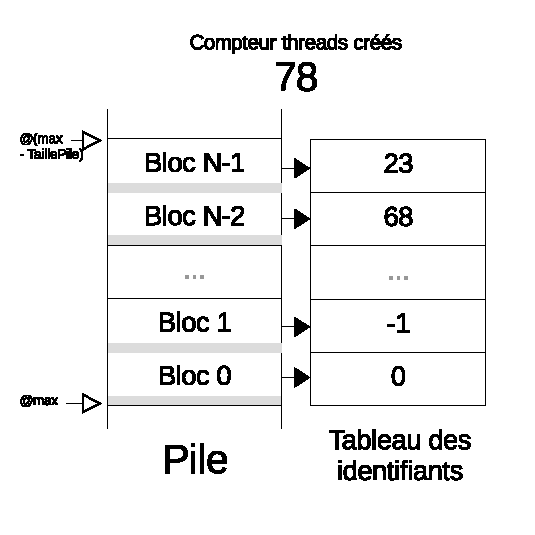
\includegraphics{schema_threads_id.eps}
				  \caption{Structures de gestion de l’identifiant de thread.}
			\end{figure}
			~\par{La pile est divisée en un nombre de blocs déterminé par le nombre de pages par thread. l'identifiant en pile représente le numéro du bloc de la pile qui est alloué au thread. Les blocs de pile sont numérotés de $0$ à $N-1$. $N-1$ étant le bloc ayant l'adresse de pile la plus petite, et $0$ le bloc ayant l'adresse la plus grande. Un thread demande un bloc en pile à sa création, et le libère lorsque se termine.}
			~\par{Afin de stocker les identifiants uniques et les identifiants en pile des threads, on utilise un tableau de taille N (nombre maximal de threads dans un processus), où chaque numéro de case représente un bloc en pile, et le contenu de la case représente l'identifiant unique du thread qui est alloué actuellement dans ce bloc en pile (si positif ou nul), ou que ce dernier n'est pas alloué (négatif, -1). Voir Figure 1.}
			~\par{Afin de tester l'état d'un thread ayant pour identifiant unique \texttt{x}, on utilise les algorithmes suivants: }
				\begin{itemize}
					\item{\texttt{x} est supérieur au nombre de threads créés: } Le thread n'a jamais été créé ;
					\item{\texttt{x} est inférieur au nombre de threads créés, mais n'est pas présent dans le tableau: } Le thread a été créé, mais s'est terminé ;
					\item{\texttt{x} est inférieur au nombre de threads créés, et est présent dans le tableau à la case \texttt{i} : Le thread a été créé, et est en cours d'exécution, et le bloc en pile numéro \texttt{i} lui est alloué.}
				\end{itemize}
		\subsubsection{Implémentation du join}
			Un vecteur contenant la liste des threads en attente et l'identifiant des threads qui les attends.
				\begin{itemize}
					\item élément who : Thread qui attend
					\item élément forId : identifiant du thread que who doit attendre
				\end{itemize}
			~\par{Dès l'appel à join du thread d'id x, on ajoute la paire (thread courant, x) à la liste des threads en attente et le thread courant appel la fonction Sleep. Elle l'enlevera de la liste d'attente du scheduler pour ne pas le réveiller inutilement, c'est le thread sur lequel le join a été effectué qui reveillera ce thread lors de son appel a UserThreadExit}

	\subsection{Mémoire virtuelle}
		\subsubsection{Pagination mémoire}
			le frame provider, utilise une bitmap et toutes les fonction implémentées pour celle-ci. La fonction de recherche d'un bit vide nous est utilisé pour aller chercher une page vide et son adresse. Et la fonction retournant le nombre de bit a 0 est utilisé pour avoir le nombre de page libre. La fonction libérant les pages utilise la fonction des bitmaps pour libérer le bit correspondant dans la bitmap.\\
			nous avons pu remarqué qu'avec la façon dont nous avons implémenté notre table de page : ppn (physical page number) = vpn (virtual page number) + 128 (taille d'une page)
				-> ceci est une faille de sécurité car elle permet de faire d'aller écrire à des endroit où l'on ne devrait pas pouvoir.
				-> cette implémntation permet tout de même d'avoir tous les autres avantages des pages virtuelles\\
			Lorsque quelque chose demande de la mémoire (création d'un process, enregistrement d'un fichier...), la bitmap nous donne une adresse puis l'adresse de la page est donée au programme pour qu'il puisse y inscrire ce dont il a besoin.\\
			Lors de la fin du programme, la(les) page(s) est déclarée(s) vide et le bit correspondant est remit à 0.
		\subsubsection{Implémentation de Fork et ForkExec}
			{Ces deux fonctions sont inspiré de StartProcess. Elles font appel à l'appel system \texttt{do\_UserProcessCreate}. ce dernier va ouvrir l'executable, lui allouer de la mémoire (un addrspace). Il va ensuite créer le thread et y attacher la mémoire allouée. Il va enfin mettre à jour le nombre de processus créés.
			\\ /!/ForkExec le thread créé sur StartUserProcess/!/
			\\ La différence entre ForkExec et Fork est que ForkExec ne mets pas la mémoire à la même adresse que celle du thread en cours.
			\\ Avant de se fermer, la machine attend la fin du dernier process. Pour savoir si le processus actuel est le dernier, la machine garde un compteur du nombre de processus en cours de fonctionement, qui est incrémenté quand un process est créer et qui est décrémenté quand un process se termine. Le dernier process est donc celui qui met le compteur a $0$ en se terminant.}

	\subsection{système de fichier}
la position dans les dossier n'est pas sauvegarder entre deux éxécutions.
lorsque la machine s'arrète, on reviens à la racine.

	\subsection{réseaux}
		Une tentative d'envoi ne se termine que lorsqu'il un message reçoit son acquittement ou qu'il ait été renvoyé (TEMPO*MAXREEMISSIONS) fois. ON ne peu attendre de message d'acquitement que pour un seul message à la fois. Pour ce faire, on utikisse un deamon qui est bloqué au départ, puis lancé dès que l'on tente d'envoyer un message puis rebloqué lorsque la tentative se fini.
		le type du message est précisé dans son header. Il peux s'agir soit d'un message normal (MSG), soit d'un message d'acquitement (ACK)
		la faiblesse de ce système est que les sygnaux d'acquitement peuvent être perdu facilement. Par exemple si une machine s'éteint en ayant envoyé un ACK qui sera perdu, l'expéditeur retentera d'envoyer le message à l'infini.
		pour transferer les fichiers, un premier paquet est envoyé contenant la taille du fichier à envoyer. puis l'envoie est fragmenté en plusieurs paquets de MaxStringSize si la taille du fichier supérieure à cette limite utilisateur. Le récépteur met tous les paquet dans un buffer dont la taille est définie par le contenu du premier paquet, pusi écrit le contenu du buffer dans un fichier.
		

\section{Organisation du travail}
	\subsection{Fonctionement du groupe}
		Malik : code/debug/docs\\
		Amine : code/docs\\
		Sebastien : code/docs\\
		Jean-Yves : organisation/docs/tests\\

	\subsection{Planning}
	\begin{itemize}
		\item semaine 1 :
			\subitem mise en place du projet
			\subitem nous avons commencé par faire la partie 1 chacun de notre coté,
			\subitem puis nous avons tous travaillé ensemble sur les parties 2 puis 3.

		\item semaine 2 :
			\subitem cette semaine, nous avons commencer par finir la partie 3
			\subitem puis nous avons enchainé sur la partie 4.

		\item semaine 3 :
			\subitem Malik : partie 5
			\subitem Amine : partie 6
			\subitem Sebastien : débug partie 4 et 5
			\subitem Jean-Yves : travail de mise en page et avancement du rapport

		\item semaine 4 :
			\subitem lundi/mardi : fin des partie 5 et 6 et debug du reste
			\subitem mercredi : fin du rapport (mise en page + schema + correction de contenu) et préparation du contenu de la présentation
			\subitem jeudi : entrainement pour la présentation
			\subitem vendredi : D-day
	\end{itemize}

\end{document}
